\chapter{Discussion}
\label{c:discussion}
\IMRADlabel{discussion}



In this chapter we will analyze the results from~\autoref{c:experiments} and set them into context with results from related work. We will discuss the performance on the different environments first and then compare our results with the results of some related work.

\section{Model Performance}
	\subsection{Proof-of-Concept: LGDS}
		As we have seen in~\autoref{fig:lgdsRollout}, the \ac{lgds} proof-of-concept environment works pretty well and the prediction perfectly matches the true data. The model has an \ac{nrmse} of approximately \( 0.0001 \) for every metric. This shows that we are still able to learn linear dynamical systems. We expected this result as we have proven that our algorithm is equivalent to the \ac{lgds} inference algorithm for linear systems in~\autoref{app:ngkExactness}. Hence, our algorithm does not reduce the "power" of the linear algorithm on linear systems and only extends its usability to nonlinear systems.
	% end

	\subsection{Pendulum}
		\label{subsec:discussPendulum}

		The pendulum is the first nonlinear environment we assess.

		As we have seen in the experiment for different latent dimensionalities, we need at least ten latent dimensions to model the pendulum with a decent prediction error, where we expected some downsides on the prediction and expected a really good rollout in the training area. As we have seen in the results for a ten-dimensional latent in~\autoref{subsubsec:pendulumL10}, we see a good rollout in the training area and also a good prediction for the pendulum position, but a slightly smaller amplitude in the velocity plot. This corresponds to an energy loss of the pendulum that should not happen as it is undamped.~\autoref{fig:pendulumEnergyL10} highlights this by showing the total, kinetic and potential energy of the system, where the rollout energy changes with time which should not happen. However, the potential energy almost matches the true potential energy, supporting our inspection that the angular displacement is well fit. The kinetic energy generated by the velocity is, on the other hand, a bit off. We can further inspect this behavior by looking at the rollout in the latent space in~\autoref{fig:pendulumLatentRolloutL10}. We see that the energy loss is primarily happening in the tenth dimension. Looking at the real parts of the eigenvalues of the latent state dynamics matrix,
		\begin{equation*}
			\sigma = \{ 1.00, 1.00, 1.00, 0.96, 0.65, 0.67, 0.86, 0.80, 0.73, 0.75 \}
		\end{equation*}
		we see that not all are close to one, \ie they vanish after some time. This directly corresponds to the energy loss in the system (the eigenvalues of a system capture the time evolution). We also see that the tenth dimension has a really high variance in its states, indicating that the model already has enough latent dimensions to explain the dynamics. Looking at the rollout of a nine-dimensional latent (run \texttt{58}) in~\autoref{fig:pendulumRolloutL09}, however, we see that the energy loss is still there. It does not make sense to inspect higher-dimensional latent spaces as we have seen in the latent dimensionalities experiment that the error does not shrink much. Additionally, the 14-dimensional latent that we inspected in~\autoref{subsubsec:pendulumL10} also looses energy. We do not expect this to get better with higher latent dimensionalities. Also, higher dimensionalities impose numerical instability, a phenomenon we will address in~\autoref{subsec:discussPerformanceNumerics}.

		For this environment, we get really small confidences with the true trajectory still being in the region of confidence. We also see that the variance is higher on the turns of the pendulum which makes sense as that is the most critical part of the movement.

		While these first results cast a shadow on our model performance, the energy loss builds hope for the damped pendulum to work out well.

		\begin{figure}
			\centering
			\begin{subfigure}{0.7\linewidth}
				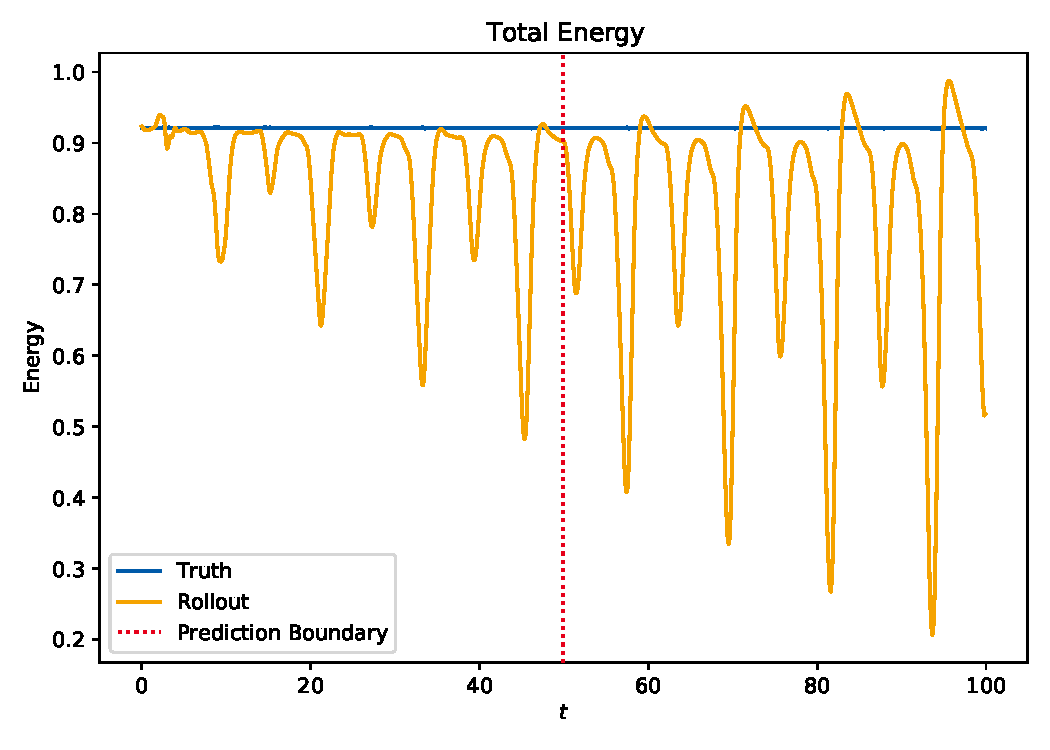
\includegraphics[width=\linewidth]{figures/results/pendulum/run-latent-dim-10/energy-R10-N0-total.png}
			\end{subfigure} \\
			\begin{subfigure}{0.5\linewidth}
				\centering
				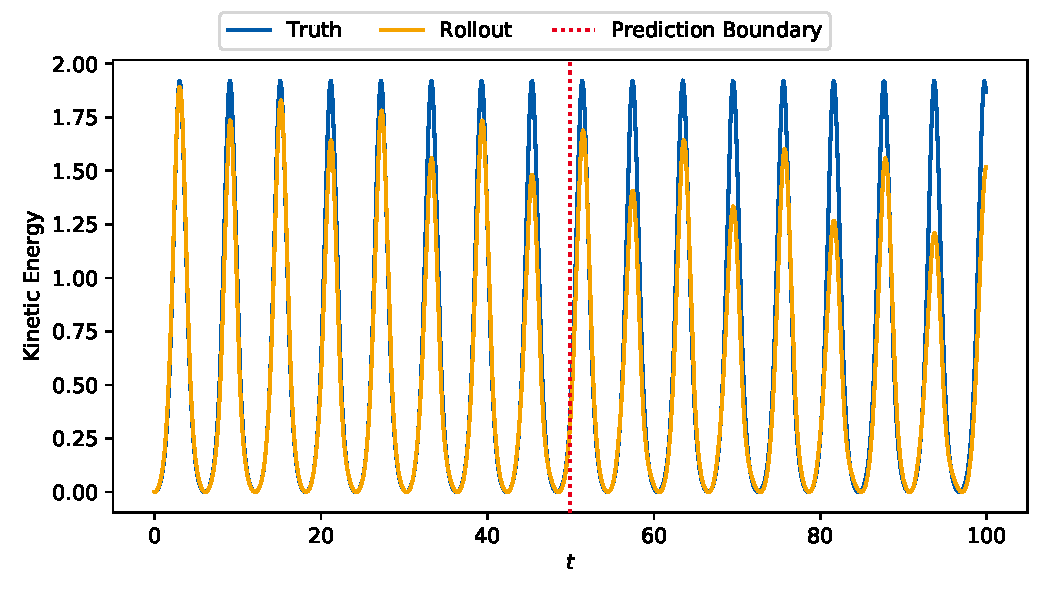
\includegraphics[width=\linewidth]{figures/results/pendulum/run-latent-dim-10/energy-R10-N0-kinetic.png}
			\end{subfigure}%
			~
			\begin{subfigure}{0.5\linewidth}
				\centering
				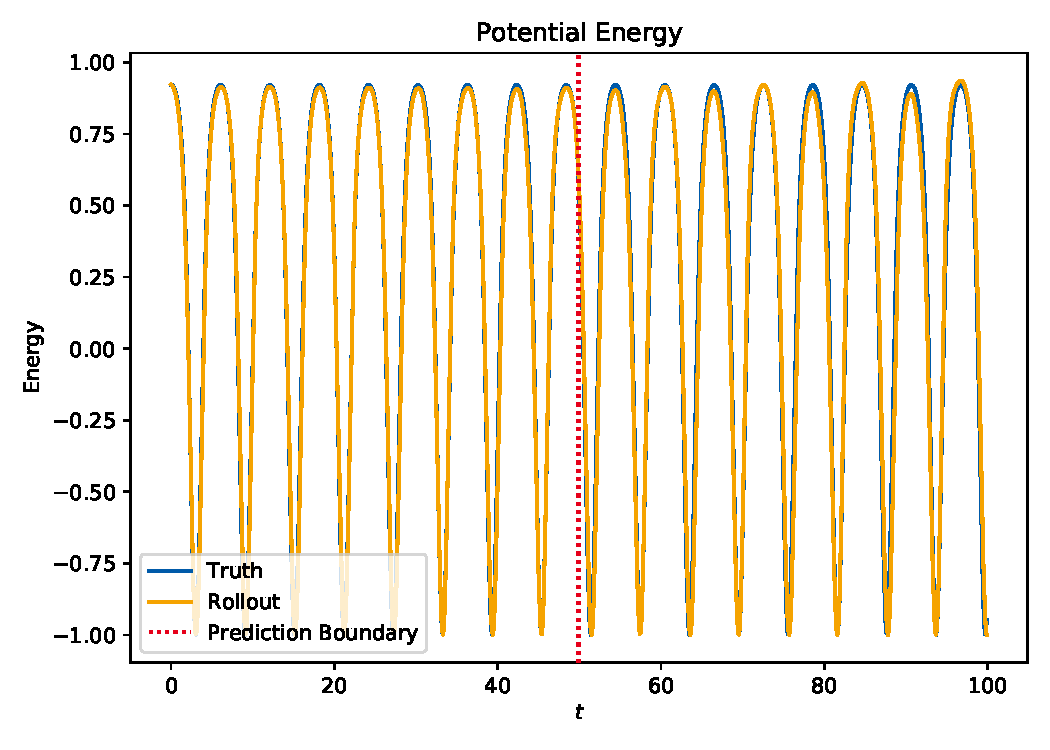
\includegraphics[width=\linewidth]{figures/results/pendulum/run-latent-dim-10/energy-R10-N0-potential.png}
			\end{subfigure}
			\caption[Total energy of the undamped pendulum]{Total energy of the undamped pendulum composed of the kinetic energy on the bottom left and the potential energy on the bottom right. The blue line represents the true energy, calculated from the training and validation data. The orange line is the energy calculated from the rollout. As usual, the red line is the prediction boundary up until all training data was used; afterwards, the model predicted the rest of the data.}
			\label{fig:pendulumEnergyL10}
		\end{figure}

		\begin{figure}
			\centering
			\includegraphics[width=\linewidth]{figures/results/pendulum/run-latent-dim-10/rollout-latents-N0.png}
			\caption[Latent rollout of the pendulum experiment for 10 latent dimensions]{Rollout of the latent dimensions of the pendulum environment for \(k = 10 \) latents.}
			\label{fig:pendulumLatentRolloutL10}
		\end{figure}

		\begin{figure}
			\centering
			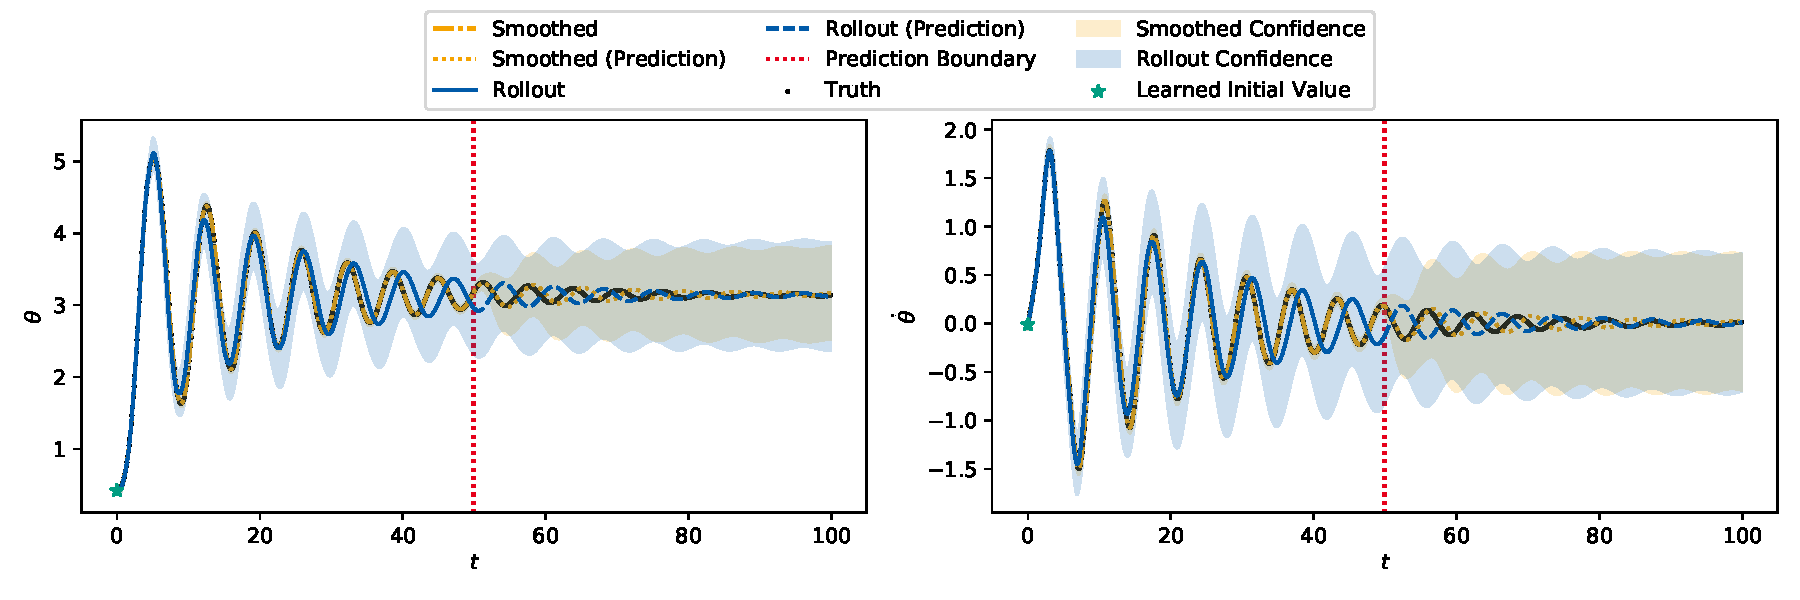
\includegraphics[width=\linewidth]{figures/results/pendulum/run-latent-dim-09/rollout-observations-N0.png}
			\caption[Rollout of the pendulum experiment for 9 latent dimensions]{The rollout plot in the observation space of the pendulum environment for \(k = 9\). The left plot shows the displacement and the right plot the angular velocity. The black dots represent the true data of which the model used everything till the red prediction boundary to train on. The blue line is the rollout, starting from the learned initial value (marked with a green star). The orange dash-dotted line is the smoothed data. The dotted orange line then is the rollout starting from the last smoothed state, forming the "smoothed prediction". The shaded regions show the confidence, \ie two times the standard deviation.}
			\label{fig:pendulumRolloutL09}
		\end{figure}
	% end

	\subsection{Damped Pendulum}
		\label{subsec:discussDampedPendulum}

		As for the undamped pendulum, we have seen in the experiment with different latent dimensionalities that we need at least ten latent dimensions. For ten dimensions, we get a decent \ac{nrmse} on both training and prediction. We have seen this behavior in~\autoref{subsubsec:pendulumDampedL10} and in the rollout plot in~\autoref{fig:pendulumDampedRolloutL10}. In contrast to the undamped pendulum, the amplitudes of the oscillations are now on the correct heights, so we definitely learn the energy loss of the system. We can also see this behavior in the plot of the total, kinetic and potential energy in~\autoref{fig:pendulumDampedEnergyL10}. We see in the total and the kinetic and potential energy that the damped pendulum model is really close to the real energy levels, in all energy types. This supports the first interpretation of the rollout that we really learn the energy loss. On the other hand, the rollout is phase-shifted to the real trajectory, sometimes even predicting the pendulum to be on the opposite side of a swing. Looking at the rollout in the latent space in~\autoref{fig:pendulumDampedLatentRolloutL10}, we see a similar behavior in the latent space, so our learned observation function seems to be correct, but the latent dynamics are a bit off.

		Improving this might be possible by fixing the observation function and optimizing just the state dynamics matrix on its own. This reduces the parameters the algorithm has to learn by a lot, possibly yielding a more accurate rollout. But overall we are satisfied with this result as we learn the energy loss and get a confidence that is not too high such that the real position is still in the region of variance. As for the undamped pendulum, we get higher variances in regions where the pendulum turns over.

		As the rollout is generated from a linear system in the background, it makes sense that energy-loosing systems can are easier to model: Taming a linear system to keep its energy for a long time is a lot harder than "letting it converge to zero". A stable non-zero system corresponds to eigenvalues that are approximately one (as \( \lim_{k \to \infty} 1^k = 1 \) and \( \lim_{k \to \infty} x^k = 0 \) for \( \lvert x \rvert < 1 \), but \( \lim_{k \to \infty} x^k \to \infty \) for \( x > 0 \)). Small disturbances to a system with eigenvalues close can cause the system to diverge quickly.

		\begin{figure}
			\centering
			\begin{subfigure}{0.7\linewidth}
				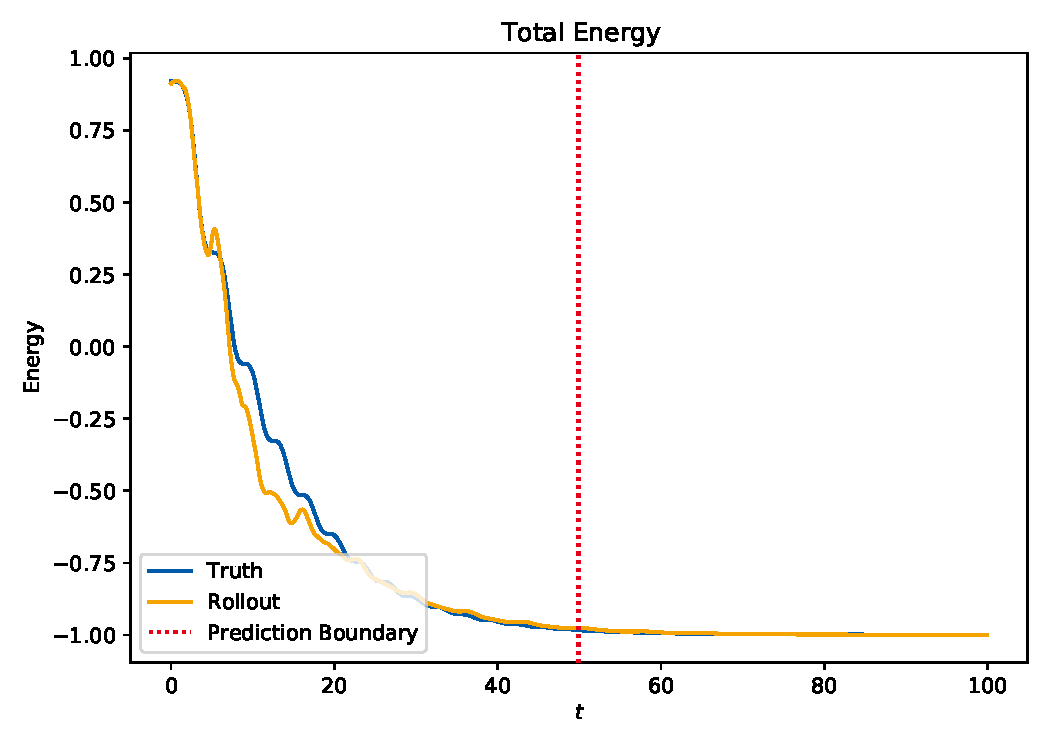
\includegraphics[width=\linewidth]{figures/results/pendulum-damped/run-latent-dim-10/energy-R110-N0-total.png}
			\end{subfigure} \\
			\begin{subfigure}{0.5\linewidth}
				\centering
				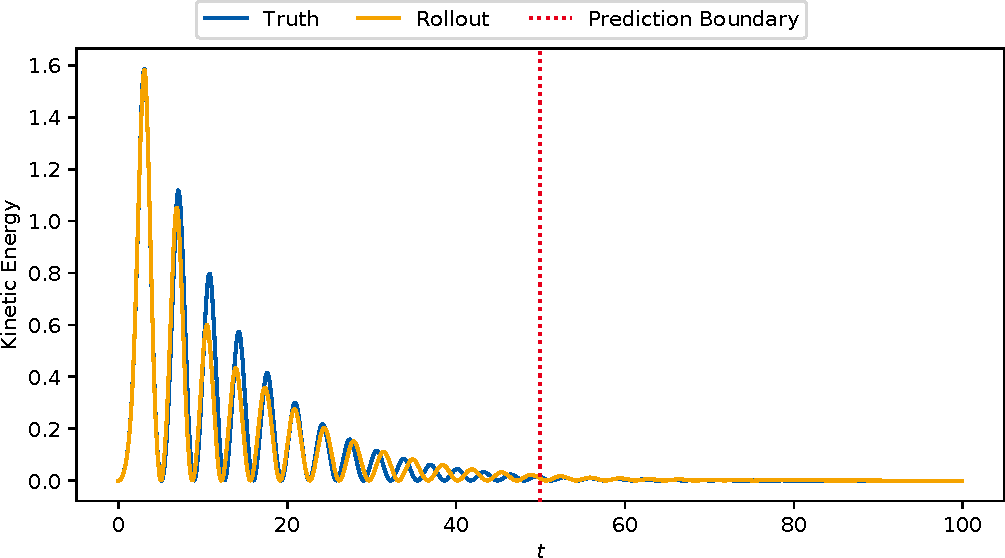
\includegraphics[width=\linewidth]{figures/results/pendulum-damped/run-latent-dim-10/energy-R110-N0-kinetic.png}
			\end{subfigure}%
			~
			\begin{subfigure}{0.5\linewidth}
				\centering
				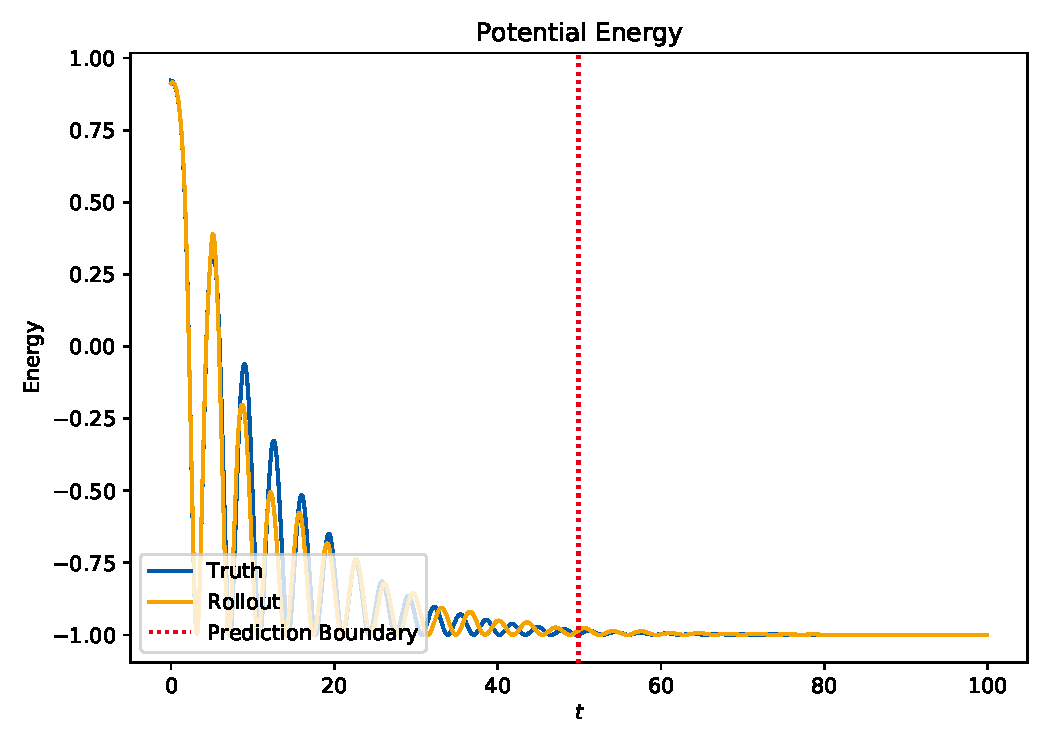
\includegraphics[width=\linewidth]{figures/results/pendulum-damped/run-latent-dim-10/energy-R110-N0-potential.png}
			\end{subfigure}
			\caption[Total energy of the damped pendulum]{Total energy of the damped pendulum composed of the kinetic energy on the bottom left and the potential energy on the bottom right. The blue line represents the true energy, calculated from the training and validation data. The orange line is the energy calculated from the rollout. As usual, the red line is the prediction boundary up until all training data was used; afterwards, the model predicted the rest of the data.}
			\label{fig:pendulumDampedEnergyL10}
		\end{figure}

		\begin{figure}
			\centering
			\includegraphics[width=\linewidth]{figures/results/pendulum-damped/run-latent-dim-10/rollout-latents-N0.png}
			\caption[Latent rollout of the damped pendulum experiment for 10 latent dimensions]{Rollout of the latent dimensions of the damped pendulum environment for \(k = 10 \) latents.}
			\label{fig:pendulumDampedLatentRolloutL10}
		\end{figure}
	% end

	\subsection{Gym Pendulum}
		\label{subsec:discussGymPendulum}

		As we have seen in the experiment with different latent dimensionalities in~\autoref{subsubsec:gymPendulumLatents}, we need at least seven latent dimensions to get a decent \ac{nrmse} on the training rollout. However, we noticed that we get better results in one run for four latent dimensions (see~\autoref{subsubsec:gymPendulumL04}) which we looked at for a comparison with~\cite{mortonDeepVariationalKoopman2019a}. This shows that our algorithm is extremely sensitive to the initialization as the neural network is initialized randomly. Looking at the rollout of the seven-dimensional latent run in~\autoref{subsubsec:gymPendulumL07}, we see that the latent "stops to change" after the prediction boundary in comparison to the four-dimensional latent where the rollout still moves (and roughly captures the dynamics). By taking a look at the rollout in the latent space in~\autoref{fig:gymPendulumLatentRolloutL04} and~\autoref{fig:gymPendulumLatentRolloutL07} for the four- and seven-dimensional run, we see completely different time behaviors.

		As we have already outlined in~\autoref{subsec:discussDampedPendulum}, it is hard for a linear system to be stable when not converging to zero. We see such a behavior in the latent rollout: While the latents of the four-dimensional run all rise exponentially after the prediction horizon, causing movement in the observation space, approximately half of the latents in the seven-dimensional exponentially increase while the other half decreases exponentially. This seems to lead to vanishing within the neural network, explaining the non-movement in the observation space. This behavior might be improved by regularizing the latent dynamics to a system with eigenvalues really close to one, leading to more stable dynamics. Another idea would be to make the latent dynamics time-dependent so compensate for the exploding states by adding an extra latent state just representing the time step. However, this would impose other difficulties and would make the system non-autonomous.

		Another interesting result of the Gym pendulum experiment is that it performs a lot worse than the simple angular pendulum in~\autoref{subsec:discussPendulum}. This might be caused by the sine/cosine terms as these add more nonlinearity to the system (with small angle approximations it is possible to model the pendulum for small displacements, this is not possible using the sine/cosine of the angle). But as taking the sine/cosine of the angle is actually a nonlinear feature transformation typically used to implicitly encode the symmetries in a polar coordinate environment like the pendulum (swinging the pendulum around one time does not increase the angle by \(2\pi\), instead the pendulum works like a congruence class generalized to \(\R\)), we could use the inverse feature transformation to recover the angle from the sine/cosine data and get a similar performance as for the angular pendulum.

		\begin{figure}
			\centering
			\includegraphics[width=\linewidth]{figures/results/pendulum-gym/run-latent-dim-04/rollout-latents-N0.png}
			\caption[Latent rollout of the Gym pendulum experiment for 6 latent dimensions]{Rollout of the latent dimensions of the Gym pendulum environment for \( k = 6 \) latents.}
			\label{fig:gymPendulumLatentRolloutL04}
		\end{figure}
		\begin{figure}
			\centering
			\includegraphics[width=\linewidth]{figures/results/pendulum-gym/run-latent-dim-07/rollout-latents-N0.png}
			\caption[Latent rollout of the Gym pendulum experiment for 7 latent dimensions]{Rollout of the latent dimensions of the Gym pendulum environment for \( k = 7 \) latents.}
			\label{fig:gymPendulumLatentRolloutL07}
		\end{figure}
	% end

	\subsection{Gym Cartpole}
		As we have seen in the experiments with different latent dimensionalities in~\autoref{subsubsec:cartpoleLatents}, we need at least ten latent dimensions to get a decent \ac{nrmse} on the (training) rollout. We have also seen that more latent dimensions (\eg 16 dimensions in~\autoref{subsubsec:cartpoleL16}) do not yield better results than ten latent dimensions (see~\autoref{subsubsec:cartpoleL10}). However, in both cases we get a near-to-perfect rollout before the prediction boundary but fail at the prediction. For the ten dimensional latent, the model captures the dynamics of the pole displacement/velocity and also the cart velocity after the prediction boundary roughly, but for the cart position the trajectory is quite off. Another interesting result is that the model is a lot more confident in the pole displacement and velocity than the cart position. Looking at just the data in~\autoref{fig:envCartpoleGym}, this makes sense. The movement of the car is more complex as it accelerates nonlinearly only through the movement of the pendulum. This does not impose a linear movement on the cart, but rather it is centered around zero with a light shifting occurring when the pendulum falls down or swings up\footnote{See \href{https://github.com/fdamken/bachelors-thesis/blob/b5a4acbc1d10fa0224a73201995222690d2fb6de/thesis/figures/cartpole.gif}{GitHub} for a GIF of the cartpole movement.}. Also, as we have seen in~\autoref{subsec:discussPendulum} and~\autoref{subsec:discussDampedPendulum}, we are able to learn the movement of an undamped and a damped pendulum, where the motion of the pole on a cart can be seen as a slightly damped pendulum as the system is transferring energy from the pendulum to the cart.
	% end

	\subsection{Gym Double Pendulum}
		As we have seen in the experiment with different latent dimensionalities, we need at least 18 latent dimensions to model the double pendulum adequately in the training rollout. As expected from the \ac{nrmse}, we get a decent fit on the rollout for 18 latent dimensions (see~\autoref{fig:acrobotRolloutL18}), but the prediction is far off the true trajectory. The prediction does not even capture the dynamics roughly and also it is pretty certain on its wrong trajectory. This matches our expectations as the double pendulum is a chaotic environment with nonlinear coupling that is really hard to learn.

		Improving the performance on the double pendulum might be possible by using a shorter integration interval \(h\) to provide the algorithm more information between the states such that it can better extrapolate from the data. Another idea, similar to the one outlined in~\autoref{subsec:discussGymPendulum}, would be to apply an inverse feature transform on the sine/cosine of the angles to reduce the dimensionality of the observation space and let "the model discover the symmetries". We will discuss this again in~\nameref{sec:futureWork}. But overall we are satisfied that we managed to learn at least the rollout on the training data even in a chaotic system.
	% end

	\subsection{Running on the CPU or GPU Makes a Difference}
		\label{subsec:cpuGpu}

		We noticed that running our code on the \ac{cpu} or on the \ac{gpu} makes a huge difference in the quality of the results, where running on the \ac{gpu} is better. The environment we noticed the greatest difference is the double pendulum, of which we added two plots in~\autoref{app:plotsCpuGpu}.~\autoref{fig:cpuVsGpuCpu} shows the double pendulum experiment result running on the \ac{cpu} and~\autoref{fig:cpuVsGpuGpu} shows the double pendulum experiment result running on the \ac{gpu}. We expect both plots to be the same, but in fact the plot of the experiment running on the \ac{cpu} looks better. These runs are the runs \texttt{1564} and \texttt{1565}, respectively. In both cases we set the seed for both NumPy and PyTorch to the same value. As the data was generated beforehand, the Gym seed does not matter in this case. We expect this to be an issue with a gradient flowing too far through the computation graph or an issue with floating point operations working differently on the \ac{cpu}/\ac{gpu}.
	% end

	\subsection{Learning Multiple Sequences at Once}
		\label{subsec:singleMulti}

		We derived the Koopman inference algorithm in a way such that it should be possible to learn on multiple observation sequences at once (see~\autoref{sec:ngkDerivation}). However, we noticed that the results of learning from multiple sequences at once yields worse results than learning one observation sequence. We have multiple explanations for this issue, the most probable being an error in the implementation we did not find. Another explanation is that in the single-sequence case the neural network of the observation function overfits to the training data and does not have enough "memory" to also overfit to another observation sequence and therefore breaks. This is a serious problem to address and we might be able to overcome this problem by adding noise to the input to improve generalization.

		\autoref{fig:plotsSingleSequence} and~\autoref{fig:plotsMultiSequence} show two rollouts on the damped pendulum environment, the former only learning on a single observation sequence and the latter learning on multiple sequences at once. We see that while the result of a single sequence captures the dynamics decently (see~\autoref{subsec:discussDampedPendulum} for an in-depth discussion), the model that learned on two sequences does not capture the dynamics correctly.
	% end

	\subsection{Discussion on Numerical Stability}
		\label{subsec:discussPerformanceNumerics}

		The primary thing we noticed in terms of numerical stability is the definiteness of the covariance matrices \(\mat{Q}\), \(\mat{R}\) and \(\mat{V}_0\). While this can be fixed by learning the Cholesky decomposition directly, better regularization or putting priors on the matrices (see~\autoref{sec:futureWork} for more information on these topics), we also faced singular matrices. This primarily happened for high latent dimensionalities, a phenomenon that can also be seen in the latent dimensionalities comparison plots in~\autoref{sec:results}. This is caused by the algorithm "not knowing what to do" with a latent dimension, \ie when it already has "enough" dimensions to explain the data. We could use this behavior to automatically detect which latents are important and which are not, called \emph{automatic relevance determination} (see~\autoref{subsec:ard}) for more proposals on this topic.

		With implementing the square-root filtering/smoothing in the E-step we gained a lot of numerical stability (also also speed) by not having to compute the Cholesky decomposition of every smoothed covariance.

		With all that combined, we are satisfied with the numerical stability of the Koopman inference algorithm, especially given that one of the great instabilities, singular matrices, lead to future work on automatic relevance determination.
	% end
% end

\section{Comparison with Related Work}
	In this section we will discuss the performance of the Koopman inference algorithm in the context of the results from related work, the \ac{dvk} model proposed in~\cite{mortonDeepVariationalKoopman2019a}. We used the code Morton et al. originally published along with their paper and modified it to work with the latest TensorFlow~\cite{abadiTensorFlowLargeScaleMachine2016} and applied the changes mentioned in~\cite{mortonDeepVariationalKoopman2019a} (\ie made the actions of the acrobot and cartpole environment continuous). Additionally, we removed the actuation abilities of the environments along with the control inputs to mimic the behavior of our work which currently does not work with control inputs. Our modified version can be found on GitHub\footnote{See \hrefGithubVariationalKoopman{\texttt{https://github.com/fdamken/variational-koopman}} on the branch \texttt{without-control}.}.

	We ran four different environments:
	\begin{itemize}
		\item The acrobot environment that is the same as our double pendulum environment presented in~\autoref{subsubsec:doublePendulum}.
		\item Two cartpole environments, one equal to our cartpole environment presented in~\autoref{subsubsec:cartpole} and one with sine and cosine of the pole angle displacement as it was done initially in the \ac{dvk} reference implementation.
		\item The pendulum environment that that is the same as our Gym pendulum environment presented in~\autoref{subsubsec:gymPendulum} with sine/cosine features.
	\end{itemize}
	If possible, we used the same amount of time steps during training for both our and the other model. However, due to numerical instabilities in their implementation, we had to deviate in terms of the number of time steps for some environments\footnote{The exact parameters we ran their code with can be found in the \hrefGithubVariationalKoopman{GitHub repository}.}:
	\begin{itemize}
		\item We could only use 32 steps on the cartpole as opposed to our model which used 150.
		\item We used 64 steps on the double pendulum as opposed to our model which used only 56.
	\end{itemize}
	Also, our algorithm currently only learns on one observation sequence, \ie if we learn on a sequence that covers \(T_\text{train}\) time steps, we only use \(T_\text{train}\) data points, while the \ac{dvk} model uses \(3968\) equally sized sequences. This sums up to \(253,\!952\) data points for the acrobot environment, \(126,\!976\) for the cartpole environment and \(198,\!400\) for the pendulum environment.

	We assess the performance of both models by looking at the rollout plots and evaluating the performance qualitatively, and by comparing the \acrlong{nrmse}. We compute the \ac{nrmse} along the whole trajectory, although we would like to point out that the "rollout" of \ac{dvk} is not a complete rollout as the observations on the training data are reconstructions of the learning data. That is, the rollout starts from the prediction boundary, possibly yielding better results before the boundary as if the data would be computed from the beginning. But this most probably does not affect our assessment in meaningful ways.

	We will now discuss the qualitative performance on each environment separately and afterwards assess the quantitative results for all environments at once.

	\subsection{Pendulum}
		The rollout on the pendulum environment of the \ac{dvk} model is shown in~\autoref{fig:mortonPendulum}. We compare these results with both our results for the Gym pendulum (with sine/cosine) features and our results on the angular pendulum. As discussed in~\autoref{subsec:discussGymPendulum}, we can assume an inverse feature transformation back to the polar coordinate space.

		We see that the reconstruction before the prediction boundary works quite well, however, the sine feature of the angle has a dent around \( t \approx 25 \). In comparison to our rollout in~\autoref{fig:gymPendulumRolloutL04} (on the Gym pendulum), our rollout in the training error before the prediction boundary matches the data better. However, the prediction of the \ac{dvk} model captures the behavior of the system better than our prediction. Looking at the angular pendulum in~\autoref{fig:pendulumRolloutL10} (on ten latent dimensions), our model captures both the dynamics before and after the prediction boundary better than the \ac{dvk} model.

		\begin{figure}
			\centering
			\includegraphics[width=\linewidth]{figures/discussion/morton/pendulum/morton-predictions.png}
			\caption[Rollout of the pendulum environment of the DVK model]{Rollout of the pendulum environment of the \ac{dvk} model, generated by us. The top row shows the sine/cosine of the displacement of the pendulum, the bottom plot shows the angular velocity. The black dots show the ground truth of the trajectory, the solid blue line the reconstructed states from the latents, the dashed blue line the prediction of the model and the shaded region shows the min-to-max distance. This is generated by sampling multiple sequences from the model and taking the maximal and minimal values at each time step. This can be roughly interpreted as the model confidence. The blue line is the mean of the sampled predictions. As usual, the red line is the prediction boundary, until which the blue line represents the reconstruction; afterwards, the model predicted the rest of the data.}
			\label{fig:mortonPendulum}
		\end{figure}
	% end

	\subsection{Cartpole}
		For the cartpole environment, we now have two versions of the environment for the \ac{dvk} model: One that uses the angle of the pole displacement directly with the rollout in~\autoref{fig:mortonCartpoleAngle} and one that uses sine/cosine features of the angle in~\autoref{fig:mortonCartpoleSineCosine}.

		We see that both the reconstruction and the prediction for both cases diverge greatly from the true data. Interestingly, in case of the sine/cosine features, the prediction diverges more from the true data compared to the angular features, even though the former was a modification originally done in the \ac{dvk} model. But we have to point out that we were not able to fully reproduce the original results, so the original version might have yielded better results. Compared to our result in~\autoref{fig:cartpoleRolloutL10} (on ten latent dimensions), our model captures the dynamics more accurately in the training section, but worse after the boundary (\ie for prediction), especially in the cart position and velocity. Overall, we can say from this qualitative comparisons, that our model performs better on the cartpole\footnote{Note that we used more time steps for training our model, but overall less data points. Also we were not able to train the \ac{dvk} model on more time steps as it became numerically unstable.}.

		\begin{figure}
			\centering
			\includegraphics[width=\linewidth]{figures/discussion/morton/cartpole/morton-predictions.png}
			\caption[Rollout of the cartpole environment of the \ac{dvk} model with angular features]{Rollout of the cartpole environment of the \ac{dvk} model with angular features, generated by us. The top row shows the position/velocity of the cart, the bottom row shows the angle and angular velocity of the pole one the cart. The black dots show the ground truth of the trajectory, the solid blue line the reconstructed states from the latents, the dashed blue line the prediction of the model and the shaded region shows the min-to-max distance. This is generated by sampling multiple sequences from the model and taking the maximal and minimal values at each time step. It can be roughly interpreted as the model confidence. The blue line is the mean of the sampled predictions. As usual, the red line is the prediction boundary, until which the blue line represents the reconstruction; afterwards, the model predicted the rest of the data.}
			\label{fig:mortonCartpoleAngle}
		\end{figure}
		\begin{figure}
			\centering
			\includegraphics[width=\linewidth]{figures/discussion/morton/cartpole-sinecosine/morton-predictions.png}
			\caption[Rollout of the cartpole environment of the \ac{dvk} model with sine/cosine features]{Rollout of the cartpole environment of the \ac{dvk} model with angular features, generated by us. The top row shows the position/velocity of the cart, the middle row shows the cosine/sine of displacement and the bottom row shows the angular velocity of the pole on the cart. The black dots show the ground truth of the trajectory, the solid blue line the reconstructed states from the latents, the dashed blue line the prediction of the model and the shaded region shows the min-to-max distance. This is generated by sampling multiple sequences from the model and taking the maximal and minimal values at each time step. It can be roughly interpreted as the model confidence. The blue line is the mean of the sampled predictions. As usual, the red line is the prediction boundary, until which the blue line represents the reconstruction; afterwards, the model predicted the rest of the data.}
			\label{fig:mortonCartpoleSineCosine}
		\end{figure}
	% end

	\subsection{Double Pendulum}
		The final environment we benchmarked on the \ac{dvk} model is the double pendulum, for which both we and the \ac{dvk} model used cosine/sine feature transformations. The rollout of the \ac{dvk} model is shown in~\autoref{fig:mortonAcrobot}.

		We see that the reconstruction and prediction of the angular velocity is quite accurate as well as the reconstruction and prediction of the sine of both angles. However, the cosine only matches some of the data points. Compared to our rollout in~\autoref{fig:acrobotRolloutL18} (on 18 latent dimensions), the reconstruction is worse but the prediction is a lot more accurate than ours on every dimension.

		\begin{figure}
			\centering
			\includegraphics[width=\linewidth]{figures/discussion/morton/acrobot/morton-predictions.png}
			\caption[Rollout of the double pendulum environment of the \ac{dvk} model]{Rollout of the double pendulum environment of the \ac{dvk}, generated by us. The top row shows the cosine/sine of the displacement of the inner pendulum, the middle row shows the cosine/sine of the displacement of the outer pendulum and the bottom row shows the angular velocities of the inner and outer pendulum, from left to right. The black dots show the ground truth of the trajectory, the solid blue line the reconstructed states from the latents, the dashed blue line the prediction of the model and the shaded region shows the min-to-max distance. This is generated by sampling multiple sequences from the model and taking the maximal and minimal values at each time step. It can be roughly interpreted as the model confidence. The blue line is the mean of the sampled predictions. As usual, the red line is the prediction boundary, until which the blue line represents the reconstruction; afterwards, the model predicted the rest of the data.}
			\label{fig:mortonAcrobot}
		\end{figure}
	% end

	\subsection{Quantitative Comparison and Summary}
		We now look at a quantitative comparison of both models, the \ac{dvk} model and the Koopman inference algorithm (ours). We use the \ac{nrmse} on the complete rollout, the rollout on the training data (or, in case of \ac{dvk}, the reconstruction) and the prediction. We summarized the different errors in~\autoref{tab:mortonComparison}, where our algorithm is almost consistently better at environments that use the angle directly instead of the cosine/sine. Also, we are almost always better in terms of the training rollout, while we perform worse in the prediction. However, these numbers should be taken with care as the \ac{nrmse} is not scale-independent (even though it is better than the \ac{rmse} due to the normalization), but as the errors reflect our results from the qualitative comparison, we are confident that our algorithm performs better.

		Overall the performance of out algorithm matched our expectations compared to the \ac{dvk} Koopman model for multiple reasons: Firstly, we gauge the uncertainty directly instead of sampling multiple trajectories and treating the min-max distance as uncertainty. Secondly, our algorithm is much more sample-efficient (see the numbers at the beginning of this section). Thirdly, as already mentioned in related work, our method has a lot simpler model in terms of number of parameters and size of neural networks. Nevertheless, the \ac{dvk} has multiple of advantages over our method: It generalizes to more environments than our approach, is numerically more stable in some senses (\eg it does not have covariance matrices that can become negative definite or singular in some cases) and it already has the ability to learn the inputs of an actuated system, as shown in~\cite{mortonDeepVariationalKoopman2019a}.

		\begin{table}
			\centering
			\begin{tabular}{c|c|c|c}
				    \textbf{Environment}      & \textbf{Error on}\dots & \textbf{Deep Variational Koopman} & \textbf{Koopman Inference} \\ \hline
				\textbf{Sine/Cosine Pendulum} &        Complete        &               0.198               &       \textbf{0.023}       \\
				        \textbf{vs.}          &        Training        &               0.168               &       \textbf{0.014}       \\
				  \textbf{Angular Pendulum}   &       Prediction       &               0.222               &       \textbf{0.029}       \\ \hline
				\textbf{Sine/Cosine Pendulum} &        Complete        &          \textbf{0.198}           &           0.200            \\
				        \textbf{vs.}          &        Training        &               0.168               &       \textbf{0.003}       \\
				\textbf{Sine/Cosine Pendulum} &       Prediction       &          \textbf{0.222}           &           0.282            \\ \hline
				  \textbf{Angular Cartpole}   &        Complete        &               0.265               &       \textbf{0.200}       \\
				        \textbf{vs.}          &        Training        &               0.466               &       \textbf{0.009}       \\
				  \textbf{Angular Cartpole}   &       Prediction       &               0.420               &       \textbf{0.377}       \\ \hline
				\textbf{Sine/Cosine Cartpole} &        Complete        &               0.470               &       \textbf{0.200}       \\
				        \textbf{vs.}          &        Training        &              17.222               &       \textbf{0.009}       \\
				  \textbf{Angular Cartpole}   &       Prediction       &               0.817               &       \textbf{0.377}       \\ \hline
				                              &        Complete        &          \textbf{0.102}           &           0.228            \\
				  \textbf{Double Pendulum}    &        Training        &               0.103               &       \textbf{0.002}       \\
				                              &       Prediction       &          \textbf{0.104}           &           0.562
			\end{tabular}
			\caption{Comparison of the errors of all environments we benchmarked DVK and Koopman inference on. The environment in the first column describes which environment the data of the DVK is collected from (before "vs.") and from which environment the data of the Koopman inference algorithm is collected from (after "vs."). The complete error is over the rollout/reconstruction over the whole sequence, the training error is over the rollout/reconstruction on the training data and prediction is over rollout on the validation data. The numbers represent the NRMSE. The respective lowest error is marked in bold font.}
			\label{tab:mortonComparison}
		\end{table}
	% end
% end

%\section{Control}  % Only if there is time left!
%	% Introduce approach to control.
%	% Show results of LGDS control which is working.
%	% Highlight difficulties.
%
%	\todo{Discussion: Control}
%% end

\section{Future Work}
	\label{sec:futureWork}

	We will now discuss and propose future work and ideas that can be tried based on the results of this thesis.

	\subsection{Control}
		In this thesis we presented a method for learning a dynamical system with no control inputs. The most obvious extension would be to add control inputs to the latent space in an additive fashion \( \vec{s}_{t + 1} = \mat{A} \vec{s}_t + \mat{B} \vec{u}_t \) with a learnable control matrix \(\mat{B}\). With this approach it might be possible to actually perform \ac{mpc} and uncertainty-aware control like in~\cite{mortonDeepVariationalKoopman2019a}, but with a simpler model. Our first approach to this would be to test this method on a simple environment like the pendulum and first learn the control rollout and afterwards perform a stabilization task and try the swing-up of the pendulum.
	% end

	\subsection{Bayesian Treatment}
		Another extension would be to employ a Bayesian view on the parameters and treat \eg the state dynamics matrix, covariance matrices and so on as random variables. This would allow to gauge the uncertainty on the dynamics itself and would allow to restrict the matrices to small ones by placing a prior on them. The approach would be to remove the \ac{ml} estimator and marginalize over the parameters to get a predictive distribution. Another semi-Bayesian approach would be to use point-estimates using a \ac{map} estimator rather than a predictive distribution.
	% end

	\subsection{Automatic Relevance Determination (ARD)}
		\label{subsec:ard}

		In combination with going full Bayesian on the model goes the implementation of automatic relevance determination of latent dimensions as proposed in~\cite{bealVariationalKalmanSmoother2000} for linear systems. Choosing a zero-mean prior might lead to a determination of non-relevant latent states, driving the state dynamics matrix to zero. Implementing this could solve the problems described in~\autoref{subsec:discussPerformanceNumerics} that the algorithm does already have "enough" latent dimensions and drives the variance to a high level on some dimensions.
	% end

	\subsection{Better Regularization and Learning the Cholesky Decomposition}
		As already outlined in~\autoref{subsubsec:implRegularization}, it might be beneficial for numerical stability to directly learn the Cholesky decomposition of the covariance matrices by using numerical optimization instead of closed-form optimization. Another approach could be to impose better regularization on the matrices if they become negative (semi-) definite. However, while giving this a short first try during our implementation, we found out that just adding some values to the diagonal does not lead to better model performance but rather drives the likelihood to negative infinity.
	% end

	\subsection{Speed Improvements by Full PyTorch or Enhanced QR Decomposition}
		As the square-root smoothing heavily uses QR decompositions which are faster on the CPU but the M-step uses backpropagation which is faster on the GPU, we had to copy the data over in every \ac{em} iteration. It might be beneficial to implement a more advanced QR decomposition (\eg~\cite{andersonCommunicationAvoidingQRDecomposition2011a}) and run the whole algorithm in the GPU.
	% end

	\subsection{(Inverse) Feature Transformations}
		As we have seen in~\ref{subsec:discussPendulum} and~\autoref{subsec:discussGymPendulum}, using the angle directly instead of the sine/cosine improves prediction capabilities a lot. It might be beneficial to try out the proposed inverse feature transformation to get the angular displacement back from the sine and cosine and to apply this technique to other environments as well (\eg the double pendulum).
	% end
% end
